\documentclass[twoside]{book}

% Packages required by doxygen
\usepackage{fixltx2e}
\usepackage{calc}
\usepackage{doxygen}
\usepackage{graphicx}
\usepackage[utf8]{inputenc}
\usepackage{makeidx}
\usepackage{multicol}
\usepackage{multirow}
\PassOptionsToPackage{warn}{textcomp}
\usepackage{textcomp}
\usepackage[nointegrals]{wasysym}
\usepackage[table]{xcolor}

% Font selection
\usepackage[T1]{fontenc}
\usepackage{mathptmx}
\usepackage[scaled=.90]{helvet}
\usepackage{courier}
\usepackage{amssymb}
\usepackage{sectsty}
\renewcommand{\familydefault}{\sfdefault}
\allsectionsfont{%
  \fontseries{bc}\selectfont%
  \color{darkgray}%
}
\renewcommand{\DoxyLabelFont}{%
  \fontseries{bc}\selectfont%
  \color{darkgray}%
}
\newcommand{\+}{\discretionary{\mbox{\scriptsize$\hookleftarrow$}}{}{}}

% Page & text layout
\usepackage{geometry}
\geometry{%
  a4paper,%
  top=2.5cm,%
  bottom=2.5cm,%
  left=2.5cm,%
  right=2.5cm%
}
\tolerance=750
\hfuzz=15pt
\hbadness=750
\setlength{\emergencystretch}{15pt}
\setlength{\parindent}{0cm}
\setlength{\parskip}{0.2cm}
\makeatletter
\renewcommand{\paragraph}{%
  \@startsection{paragraph}{4}{0ex}{-1.0ex}{1.0ex}{%
    \normalfont\normalsize\bfseries\SS@parafont%
  }%
}
\renewcommand{\subparagraph}{%
  \@startsection{subparagraph}{5}{0ex}{-1.0ex}{1.0ex}{%
    \normalfont\normalsize\bfseries\SS@subparafont%
  }%
}
\makeatother

% Headers & footers
\usepackage{fancyhdr}
\pagestyle{fancyplain}
\fancyhead[LE]{\fancyplain{}{\bfseries\thepage}}
\fancyhead[CE]{\fancyplain{}{}}
\fancyhead[RE]{\fancyplain{}{\bfseries\leftmark}}
\fancyhead[LO]{\fancyplain{}{\bfseries\rightmark}}
\fancyhead[CO]{\fancyplain{}{}}
\fancyhead[RO]{\fancyplain{}{\bfseries\thepage}}
\fancyfoot[LE]{\fancyplain{}{}}
\fancyfoot[CE]{\fancyplain{}{}}
\fancyfoot[RE]{\fancyplain{}{\bfseries\scriptsize Generated on Mon Dec 29 2014 19\+:22\+:08 for Vixlet by Doxygen }}
\fancyfoot[LO]{\fancyplain{}{\bfseries\scriptsize Generated on Mon Dec 29 2014 19\+:22\+:08 for Vixlet by Doxygen }}
\fancyfoot[CO]{\fancyplain{}{}}
\fancyfoot[RO]{\fancyplain{}{}}
\renewcommand{\footrulewidth}{0.4pt}
\renewcommand{\chaptermark}[1]{%
  \markboth{#1}{}%
}
\renewcommand{\sectionmark}[1]{%
  \markright{\thesection\ #1}%
}

% Indices & bibliography
\usepackage{natbib}
\usepackage[titles]{tocloft}
\setcounter{tocdepth}{3}
\setcounter{secnumdepth}{5}
\makeindex

% Hyperlinks (required, but should be loaded last)
\usepackage{ifpdf}
\ifpdf
  \usepackage[pdftex,pagebackref=true]{hyperref}
\else
  \usepackage[ps2pdf,pagebackref=true]{hyperref}
\fi
\hypersetup{%
  colorlinks=true,%
  linkcolor=blue,%
  citecolor=blue,%
  unicode%
}

% Custom commands
\newcommand{\clearemptydoublepage}{%
  \newpage{\pagestyle{empty}\cleardoublepage}%
}


%===== C O N T E N T S =====

\begin{document}

% Titlepage & ToC
\hypersetup{pageanchor=false,
             bookmarks=true,
             bookmarksnumbered=true,
             pdfencoding=unicode
            }
\pagenumbering{roman}
\begin{titlepage}
\vspace*{7cm}
\begin{center}%
{\Large Vixlet \\[1ex]\large 1.\+0 }\\
\vspace*{1cm}
{\large Generated by Doxygen 1.8.8}\\
\vspace*{0.5cm}
{\small Mon Dec 29 2014 19:22:08}\\
\end{center}
\end{titlepage}
\clearemptydoublepage
\tableofcontents
\clearemptydoublepage
\pagenumbering{arabic}
\hypersetup{pageanchor=true}

%--- Begin generated contents ---
\chapter{Hierarchical Index}
\section{Class Hierarchy}
This inheritance list is sorted roughly, but not completely, alphabetically\+:\begin{DoxyCompactList}
\item N\+S\+Object\begin{DoxyCompactList}
\item \contentsline{section}{Audio\+Controller}{\pageref{d1/d60/interface_audio_controller}}{}
\end{DoxyCompactList}
\item $<$U\+I\+Application\+Delegate$>$\begin{DoxyCompactList}
\item \contentsline{section}{A\+P\+P\+App\+Delegate}{\pageref{dd/d31/interface_a_p_p_app_delegate}}{}
\end{DoxyCompactList}
\item $<$U\+I\+Page\+View\+Controller\+Data\+Source$>$\begin{DoxyCompactList}
\item \contentsline{section}{A\+P\+P\+View\+Controller}{\pageref{d3/ddb/interface_a_p_p_view_controller}}{}
\end{DoxyCompactList}
\item U\+I\+Responder\begin{DoxyCompactList}
\item \contentsline{section}{A\+P\+P\+App\+Delegate}{\pageref{dd/d31/interface_a_p_p_app_delegate}}{}
\end{DoxyCompactList}
\item U\+I\+View\+Controller\begin{DoxyCompactList}
\item \contentsline{section}{A\+P\+P\+Child\+View\+Controller}{\pageref{d0/db2/interface_a_p_p_child_view_controller}}{}
\item \contentsline{section}{A\+P\+P\+View\+Controller}{\pageref{d3/ddb/interface_a_p_p_view_controller}}{}
\end{DoxyCompactList}
\end{DoxyCompactList}

\chapter{Class Index}
\section{Class List}
Here are the classes, structs, unions and interfaces with brief descriptions\+:\begin{DoxyCompactList}
\item\contentsline{section}{\hyperlink{interface_a_p_p_app_delegate}{A\+P\+P\+App\+Delegate} }{\pageref{dd/d31/interface_a_p_p_app_delegate}}{}
\item\contentsline{section}{\hyperlink{interface_a_p_p_child_view_controller}{A\+P\+P\+Child\+View\+Controller} }{\pageref{d0/db2/interface_a_p_p_child_view_controller}}{}
\item\contentsline{section}{\hyperlink{interface_a_p_p_view_controller}{A\+P\+P\+View\+Controller} }{\pageref{d3/ddb/interface_a_p_p_view_controller}}{}
\item\contentsline{section}{\hyperlink{interface_audio_controller}{Audio\+Controller} }{\pageref{d1/d60/interface_audio_controller}}{}
\end{DoxyCompactList}

\chapter{File Index}
\section{File List}
Here is a list of all files with brief descriptions\+:\begin{DoxyCompactList}
\item\contentsline{section}{/\+Users/hubino-\/mac/\+Page\+App/\+Page\+App/\hyperlink{_a_p_p_app_delegate_8h}{A\+P\+P\+App\+Delegate.\+h} }{\pageref{d7/da3/_a_p_p_app_delegate_8h}}{}
\item\contentsline{section}{/\+Users/hubino-\/mac/\+Page\+App/\+Page\+App/\hyperlink{_a_p_p_child_view_controller_8h}{A\+P\+P\+Child\+View\+Controller.\+h} }{\pageref{d5/df3/_a_p_p_child_view_controller_8h}}{}
\item\contentsline{section}{/\+Users/hubino-\/mac/\+Page\+App/\+Page\+App/\hyperlink{_a_p_p_view_controller_8h}{A\+P\+P\+View\+Controller.\+h} }{\pageref{d3/d86/_a_p_p_view_controller_8h}}{}
\item\contentsline{section}{/\+Users/hubino-\/mac/\+Page\+App/\+Page\+App/\hyperlink{_audio_controller_8h}{Audio\+Controller.\+h} }{\pageref{d8/d23/_audio_controller_8h}}{}
\end{DoxyCompactList}

\chapter{Class Documentation}
\hypertarget{interface_a_p_p_app_delegate}{\section{A\+P\+P\+App\+Delegate Class Reference}
\label{interface_a_p_p_app_delegate}\index{A\+P\+P\+App\+Delegate@{A\+P\+P\+App\+Delegate}}
}


{\ttfamily \#import $<$A\+P\+P\+App\+Delegate.\+h$>$}

Inheritance diagram for A\+P\+P\+App\+Delegate\+:\begin{figure}[H]
\begin{center}
\leavevmode
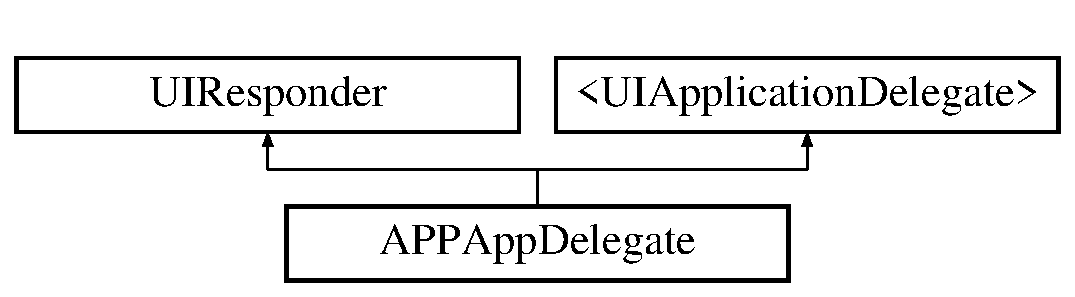
\includegraphics[height=2.000000cm]{dd/d31/interface_a_p_p_app_delegate}
\end{center}
\end{figure}
\subsection*{Properties}
\begin{DoxyCompactItemize}
\item 
U\+I\+Window $\ast$ \hyperlink{interface_a_p_p_app_delegate_a4b8f6d91c1115b02d85644fff0f447c7}{window}
\item 
\hyperlink{interface_a_p_p_view_controller}{A\+P\+P\+View\+Controller} $\ast$ \hyperlink{interface_a_p_p_app_delegate_a4c52917da489f30f98d31b4aae72a3cf}{view\+Controller}
\end{DoxyCompactItemize}


\subsection{Property Documentation}
\hypertarget{interface_a_p_p_app_delegate_a4c52917da489f30f98d31b4aae72a3cf}{\index{A\+P\+P\+App\+Delegate@{A\+P\+P\+App\+Delegate}!view\+Controller@{view\+Controller}}
\index{view\+Controller@{view\+Controller}!A\+P\+P\+App\+Delegate@{A\+P\+P\+App\+Delegate}}
\subsubsection[{view\+Controller}]{\setlength{\rightskip}{0pt plus 5cm}-\/ ({\bf A\+P\+P\+View\+Controller}$\ast$) view\+Controller\hspace{0.3cm}{\ttfamily [read]}, {\ttfamily [write]}, {\ttfamily [nonatomic]}, {\ttfamily [strong]}}}\label{interface_a_p_p_app_delegate_a4c52917da489f30f98d31b4aae72a3cf}
\hypertarget{interface_a_p_p_app_delegate_a4b8f6d91c1115b02d85644fff0f447c7}{\index{A\+P\+P\+App\+Delegate@{A\+P\+P\+App\+Delegate}!window@{window}}
\index{window@{window}!A\+P\+P\+App\+Delegate@{A\+P\+P\+App\+Delegate}}
\subsubsection[{window}]{\setlength{\rightskip}{0pt plus 5cm}-\/ (U\+I\+Window$\ast$) window\hspace{0.3cm}{\ttfamily [read]}, {\ttfamily [write]}, {\ttfamily [nonatomic]}, {\ttfamily [strong]}}}\label{interface_a_p_p_app_delegate_a4b8f6d91c1115b02d85644fff0f447c7}


The documentation for this class was generated from the following file\+:\begin{DoxyCompactItemize}
\item 
/\+Users/hubino-\/mac/\+Page\+App/\+Page\+App/\hyperlink{_a_p_p_app_delegate_8h}{A\+P\+P\+App\+Delegate.\+h}\end{DoxyCompactItemize}

\hypertarget{interface_a_p_p_child_view_controller}{\section{A\+P\+P\+Child\+View\+Controller Class Reference}
\label{interface_a_p_p_child_view_controller}\index{A\+P\+P\+Child\+View\+Controller@{A\+P\+P\+Child\+View\+Controller}}
}


{\ttfamily \#import $<$A\+P\+P\+Child\+View\+Controller.\+h$>$}

Inheritance diagram for A\+P\+P\+Child\+View\+Controller\+:\begin{figure}[H]
\begin{center}
\leavevmode
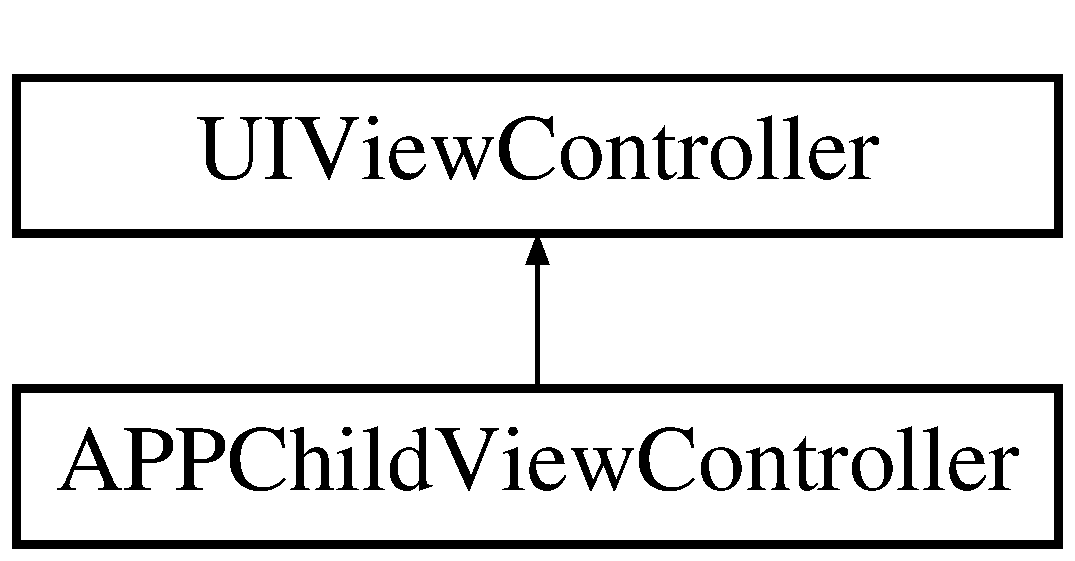
\includegraphics[height=2.000000cm]{d0/db2/interface_a_p_p_child_view_controller}
\end{center}
\end{figure}
\subsection*{Protected Attributes}
\begin{DoxyCompactItemize}
\item 
C\+G\+P\+D\+F\+Document\+Ref \hyperlink{interface_a_p_p_child_view_controller_a49090a70e7ab1989a9675acbd042eb9e}{pdf}
\end{DoxyCompactItemize}
\subsection*{Properties}
\begin{DoxyCompactItemize}
\item 
N\+S\+Integer \hyperlink{interface_a_p_p_child_view_controller_accecfd9572f912f5ca9e35236521d49a}{index}
\item 
I\+B\+Outlet U\+I\+Label $\ast$ \hyperlink{interface_a_p_p_child_view_controller_acb441c535672227c1f1f0ab06d2ab9fe}{screen\+Number}
\item 
I\+B\+Outlet U\+I\+Web\+View $\ast$ \hyperlink{interface_a_p_p_child_view_controller_a1f5838da40857d637ed5a6cf412910f8}{web\+View}
\item 
id \hyperlink{interface_a_p_p_child_view_controller_a45d2bf0ae541d2145028922b6076cdf5}{data\+Object}
\end{DoxyCompactItemize}


\subsection{Member Data Documentation}
\hypertarget{interface_a_p_p_child_view_controller_a49090a70e7ab1989a9675acbd042eb9e}{\index{A\+P\+P\+Child\+View\+Controller@{A\+P\+P\+Child\+View\+Controller}!pdf@{pdf}}
\index{pdf@{pdf}!A\+P\+P\+Child\+View\+Controller@{A\+P\+P\+Child\+View\+Controller}}
\subsubsection[{pdf}]{\setlength{\rightskip}{0pt plus 5cm}-\/ (C\+G\+P\+D\+F\+Document\+Ref) pdf\hspace{0.3cm}{\ttfamily [protected]}}}\label{interface_a_p_p_child_view_controller_a49090a70e7ab1989a9675acbd042eb9e}


\subsection{Property Documentation}
\hypertarget{interface_a_p_p_child_view_controller_a45d2bf0ae541d2145028922b6076cdf5}{\index{A\+P\+P\+Child\+View\+Controller@{A\+P\+P\+Child\+View\+Controller}!data\+Object@{data\+Object}}
\index{data\+Object@{data\+Object}!A\+P\+P\+Child\+View\+Controller@{A\+P\+P\+Child\+View\+Controller}}
\subsubsection[{data\+Object}]{\setlength{\rightskip}{0pt plus 5cm}-\/ (id) data\+Object\hspace{0.3cm}{\ttfamily [read]}, {\ttfamily [write]}, {\ttfamily [nonatomic]}, {\ttfamily [strong]}}}\label{interface_a_p_p_child_view_controller_a45d2bf0ae541d2145028922b6076cdf5}
\hypertarget{interface_a_p_p_child_view_controller_accecfd9572f912f5ca9e35236521d49a}{\index{A\+P\+P\+Child\+View\+Controller@{A\+P\+P\+Child\+View\+Controller}!index@{index}}
\index{index@{index}!A\+P\+P\+Child\+View\+Controller@{A\+P\+P\+Child\+View\+Controller}}
\subsubsection[{index}]{\setlength{\rightskip}{0pt plus 5cm}-\/ (N\+S\+Integer) index\hspace{0.3cm}{\ttfamily [read]}, {\ttfamily [write]}, {\ttfamily [nonatomic]}, {\ttfamily [assign]}}}\label{interface_a_p_p_child_view_controller_accecfd9572f912f5ca9e35236521d49a}
\hypertarget{interface_a_p_p_child_view_controller_acb441c535672227c1f1f0ab06d2ab9fe}{\index{A\+P\+P\+Child\+View\+Controller@{A\+P\+P\+Child\+View\+Controller}!screen\+Number@{screen\+Number}}
\index{screen\+Number@{screen\+Number}!A\+P\+P\+Child\+View\+Controller@{A\+P\+P\+Child\+View\+Controller}}
\subsubsection[{screen\+Number}]{\setlength{\rightskip}{0pt plus 5cm}-\/ (I\+B\+Outlet U\+I\+Label$\ast$) screen\+Number\hspace{0.3cm}{\ttfamily [read]}, {\ttfamily [write]}, {\ttfamily [nonatomic]}, {\ttfamily [strong]}}}\label{interface_a_p_p_child_view_controller_acb441c535672227c1f1f0ab06d2ab9fe}
\hypertarget{interface_a_p_p_child_view_controller_a1f5838da40857d637ed5a6cf412910f8}{\index{A\+P\+P\+Child\+View\+Controller@{A\+P\+P\+Child\+View\+Controller}!web\+View@{web\+View}}
\index{web\+View@{web\+View}!A\+P\+P\+Child\+View\+Controller@{A\+P\+P\+Child\+View\+Controller}}
\subsubsection[{web\+View}]{\setlength{\rightskip}{0pt plus 5cm}-\/ (I\+B\+Outlet U\+I\+Web\+View$\ast$) web\+View\hspace{0.3cm}{\ttfamily [read]}, {\ttfamily [write]}, {\ttfamily [nonatomic]}, {\ttfamily [strong]}}}\label{interface_a_p_p_child_view_controller_a1f5838da40857d637ed5a6cf412910f8}


The documentation for this class was generated from the following file\+:\begin{DoxyCompactItemize}
\item 
/\+Users/hubino-\/mac/\+Page\+App/\+Page\+App/\hyperlink{_a_p_p_child_view_controller_8h}{A\+P\+P\+Child\+View\+Controller.\+h}\end{DoxyCompactItemize}

\hypertarget{interface_a_p_p_view_controller}{\section{A\+P\+P\+View\+Controller Class Reference}
\label{interface_a_p_p_view_controller}\index{A\+P\+P\+View\+Controller@{A\+P\+P\+View\+Controller}}
}


{\ttfamily \#import $<$A\+P\+P\+View\+Controller.\+h$>$}

Inheritance diagram for A\+P\+P\+View\+Controller\+:\begin{figure}[H]
\begin{center}
\leavevmode
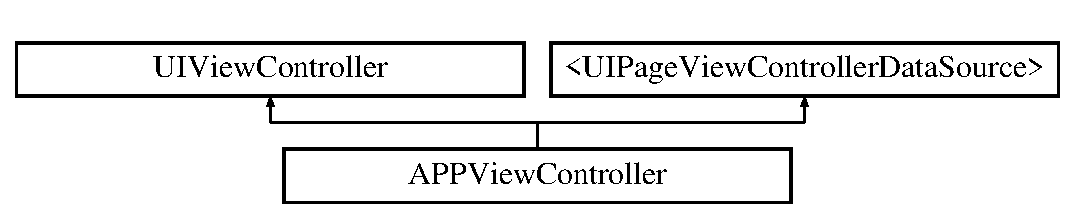
\includegraphics[height=2.000000cm]{d3/ddb/interface_a_p_p_view_controller}
\end{center}
\end{figure}
\subsection*{Properties}
\begin{DoxyCompactItemize}
\item 
U\+I\+Page\+View\+Controller $\ast$ \hyperlink{interface_a_p_p_view_controller_a5ff97842eac6699ffb211f1ea2b93f3a}{page\+Controller}
\item 
N\+S\+Array $\ast$ \hyperlink{interface_a_p_p_view_controller_ae8a6de2bf7263546c8d7edb133392da6}{page\+Content}
\end{DoxyCompactItemize}


\subsection{Property Documentation}
\hypertarget{interface_a_p_p_view_controller_ae8a6de2bf7263546c8d7edb133392da6}{\index{A\+P\+P\+View\+Controller@{A\+P\+P\+View\+Controller}!page\+Content@{page\+Content}}
\index{page\+Content@{page\+Content}!A\+P\+P\+View\+Controller@{A\+P\+P\+View\+Controller}}
\subsubsection[{page\+Content}]{\setlength{\rightskip}{0pt plus 5cm}-\/ (N\+S\+Array$\ast$) page\+Content\hspace{0.3cm}{\ttfamily [read]}, {\ttfamily [write]}, {\ttfamily [nonatomic]}, {\ttfamily [strong]}}}\label{interface_a_p_p_view_controller_ae8a6de2bf7263546c8d7edb133392da6}
\hypertarget{interface_a_p_p_view_controller_a5ff97842eac6699ffb211f1ea2b93f3a}{\index{A\+P\+P\+View\+Controller@{A\+P\+P\+View\+Controller}!page\+Controller@{page\+Controller}}
\index{page\+Controller@{page\+Controller}!A\+P\+P\+View\+Controller@{A\+P\+P\+View\+Controller}}
\subsubsection[{page\+Controller}]{\setlength{\rightskip}{0pt plus 5cm}-\/ (U\+I\+Page\+View\+Controller$\ast$) page\+Controller\hspace{0.3cm}{\ttfamily [read]}, {\ttfamily [write]}, {\ttfamily [nonatomic]}, {\ttfamily [strong]}}}\label{interface_a_p_p_view_controller_a5ff97842eac6699ffb211f1ea2b93f3a}


The documentation for this class was generated from the following file\+:\begin{DoxyCompactItemize}
\item 
/\+Users/hubino-\/mac/\+Page\+App/\+Page\+App/\hyperlink{_a_p_p_view_controller_8h}{A\+P\+P\+View\+Controller.\+h}\end{DoxyCompactItemize}

\hypertarget{interface_audio_controller}{\section{Audio\+Controller Class Reference}
\label{interface_audio_controller}\index{Audio\+Controller@{Audio\+Controller}}
}


{\ttfamily \#import $<$Audio\+Controller.\+h$>$}

Inheritance diagram for Audio\+Controller\+:\begin{figure}[H]
\begin{center}
\leavevmode
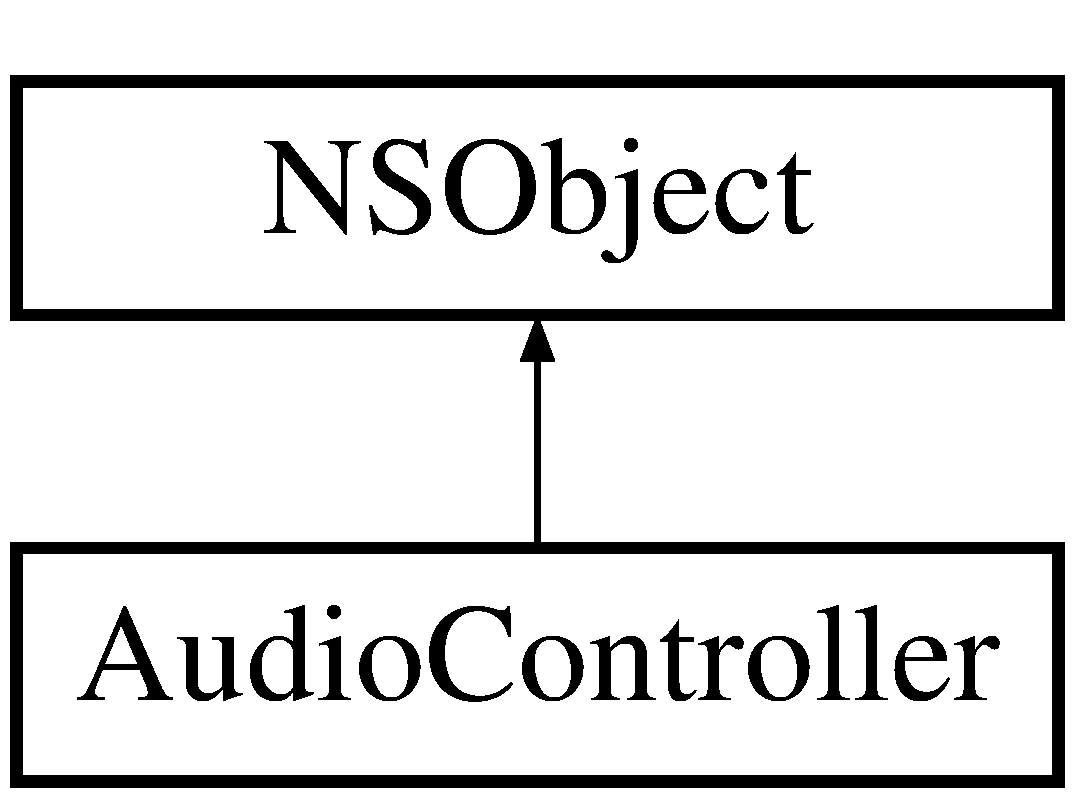
\includegraphics[height=2.000000cm]{d1/d60/interface_audio_controller}
\end{center}
\end{figure}
\subsection*{Instance Methods}
\begin{DoxyCompactItemize}
\item 
(instancetype) -\/ \hyperlink{interface_audio_controller_a7013b8ea0aded4b85246b4aac3f2aca3}{init}
\item 
(void) -\/ \hyperlink{interface_audio_controller_ad106c77329720c80a78f51b33961bfc2}{try\+Play\+Music}
\item 
(void) -\/ \hyperlink{interface_audio_controller_ab43bef477818c79902266b4064526c01}{play\+System\+Sound}
\end{DoxyCompactItemize}


\subsection{Method Documentation}
\hypertarget{interface_audio_controller_a7013b8ea0aded4b85246b4aac3f2aca3}{\index{Audio\+Controller@{Audio\+Controller}!init@{init}}
\index{init@{init}!Audio\+Controller@{Audio\+Controller}}
\subsubsection[{init}]{\setlength{\rightskip}{0pt plus 5cm}-\/ (instancetype) init 
\begin{DoxyParamCaption}
{}
\end{DoxyParamCaption}
}}\label{interface_audio_controller_a7013b8ea0aded4b85246b4aac3f2aca3}
\hypertarget{interface_audio_controller_ab43bef477818c79902266b4064526c01}{\index{Audio\+Controller@{Audio\+Controller}!play\+System\+Sound@{play\+System\+Sound}}
\index{play\+System\+Sound@{play\+System\+Sound}!Audio\+Controller@{Audio\+Controller}}
\subsubsection[{play\+System\+Sound}]{\setlength{\rightskip}{0pt plus 5cm}-\/ (void) play\+System\+Sound 
\begin{DoxyParamCaption}
{}
\end{DoxyParamCaption}
}}\label{interface_audio_controller_ab43bef477818c79902266b4064526c01}
\hypertarget{interface_audio_controller_ad106c77329720c80a78f51b33961bfc2}{\index{Audio\+Controller@{Audio\+Controller}!try\+Play\+Music@{try\+Play\+Music}}
\index{try\+Play\+Music@{try\+Play\+Music}!Audio\+Controller@{Audio\+Controller}}
\subsubsection[{try\+Play\+Music}]{\setlength{\rightskip}{0pt plus 5cm}-\/ (void) try\+Play\+Music 
\begin{DoxyParamCaption}
{}
\end{DoxyParamCaption}
}}\label{interface_audio_controller_ad106c77329720c80a78f51b33961bfc2}


The documentation for this class was generated from the following file\+:\begin{DoxyCompactItemize}
\item 
/\+Users/hubino-\/mac/\+Page\+App/\+Page\+App/\hyperlink{_audio_controller_8h}{Audio\+Controller.\+h}\end{DoxyCompactItemize}

\chapter{File Documentation}
\hypertarget{_a_p_p_app_delegate_8h}{\section{/\+Users/hubino-\/mac/\+Page\+App/\+Page\+App/\+A\+P\+P\+App\+Delegate.h File Reference}
\label{_a_p_p_app_delegate_8h}\index{/\+Users/hubino-\/mac/\+Page\+App/\+Page\+App/\+A\+P\+P\+App\+Delegate.\+h@{/\+Users/hubino-\/mac/\+Page\+App/\+Page\+App/\+A\+P\+P\+App\+Delegate.\+h}}
}
{\ttfamily \#import $<$U\+I\+Kit/\+U\+I\+Kit.\+h$>$}\\*
\subsection*{Classes}
\begin{DoxyCompactItemize}
\item 
class \hyperlink{interface_a_p_p_app_delegate}{A\+P\+P\+App\+Delegate}
\end{DoxyCompactItemize}

\hypertarget{_a_p_p_child_view_controller_8h}{\section{/\+Users/hubino-\/mac/\+Page\+App/\+Page\+App/\+A\+P\+P\+Child\+View\+Controller.h File Reference}
\label{_a_p_p_child_view_controller_8h}\index{/\+Users/hubino-\/mac/\+Page\+App/\+Page\+App/\+A\+P\+P\+Child\+View\+Controller.\+h@{/\+Users/hubino-\/mac/\+Page\+App/\+Page\+App/\+A\+P\+P\+Child\+View\+Controller.\+h}}
}
{\ttfamily \#import $<$U\+I\+Kit/\+U\+I\+Kit.\+h$>$}\\*
{\ttfamily \#import $<$Audio\+Toolbox/\+Audio\+Toolbox.\+h$>$}\\*
\subsection*{Classes}
\begin{DoxyCompactItemize}
\item 
class \hyperlink{interface_a_p_p_child_view_controller}{A\+P\+P\+Child\+View\+Controller}
\end{DoxyCompactItemize}

\hypertarget{_a_p_p_view_controller_8h}{\section{/\+Users/hubino-\/mac/\+Page\+App/\+Page\+App/\+A\+P\+P\+View\+Controller.h File Reference}
\label{_a_p_p_view_controller_8h}\index{/\+Users/hubino-\/mac/\+Page\+App/\+Page\+App/\+A\+P\+P\+View\+Controller.\+h@{/\+Users/hubino-\/mac/\+Page\+App/\+Page\+App/\+A\+P\+P\+View\+Controller.\+h}}
}
{\ttfamily \#import $<$U\+I\+Kit/\+U\+I\+Kit.\+h$>$}\\*
\subsection*{Classes}
\begin{DoxyCompactItemize}
\item 
class \hyperlink{interface_a_p_p_view_controller}{A\+P\+P\+View\+Controller}
\end{DoxyCompactItemize}

\hypertarget{_audio_controller_8h}{\section{/\+Users/hubino-\/mac/\+Page\+App/\+Page\+App/\+Audio\+Controller.h File Reference}
\label{_audio_controller_8h}\index{/\+Users/hubino-\/mac/\+Page\+App/\+Page\+App/\+Audio\+Controller.\+h@{/\+Users/hubino-\/mac/\+Page\+App/\+Page\+App/\+Audio\+Controller.\+h}}
}
{\ttfamily \#import $<$Foundation/\+Foundation.\+h$>$}\\*
{\ttfamily \#import $<$A\+V\+Foundation/\+A\+V\+Foundation.\+h$>$}\\*
{\ttfamily \#import $<$Audio\+Toolbox/\+Audio\+Toolbox.\+h$>$}\\*
\subsection*{Classes}
\begin{DoxyCompactItemize}
\item 
class \hyperlink{interface_audio_controller}{Audio\+Controller}
\end{DoxyCompactItemize}

%--- End generated contents ---

% Index
\newpage
\phantomsection
\addcontentsline{toc}{chapter}{Index}
\printindex

\end{document}
